\cleartooddpage[\thispagestyle{empty}]
\chapter{Data Visualization}\label{vis}
\moduleinfo{vis}
The ``vis'' module provides utilities for viewing data in Tcl. 
It utilizes the ``wob'' package for managing Tk widgets, so in order to interact with the widgets, one must enter the Tcl/Tk event loop. 
The \textit{mainLoop} command in the ``wob'' package is an easy way to accomplish this.

\clearpage
\section{View Tabular and Matrix Data}
Tda tables and matrices can be interactively explored with the commands \cmdlink{viewTable} and \cmdlink{viewMatrix}. 
Data can be selected and copied as CSV to paste in other applications.

\begin{syntax}
viewTable \$tblObj
\end{syntax}
\begin{syntax}
viewMatrix \$matrix
\end{syntax}
\begin{args}
\$tblObj & Object name of Tda table object. \\
\$matrix  & Matrix to view. 
\end{args}
\begin{example}{Viewing tabular and matrix data}
\begin{lstlisting}
set tblObj [tbl new]
$tblObj define data {
    1 {x 3.44 y 7.11 z 8.67}
    2 {x 4.61 y 1.81 z 7.63}
    3 {x 8.25 y 7.56 z 3.84}
    4 {x 5.20 y 6.78 z 1.11}
    5 {x 3.26 y 9.92 z 4.56}
}
viewTable $tblObj
viewMatrix [$tblObj values]
wob::mainLoop
\end{lstlisting}
\end{example}
\begin{figure}[!htb]
\centering
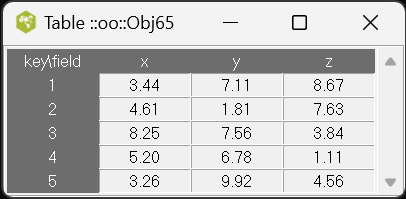
\includegraphics[width=0.4\linewidth]{viewtable}
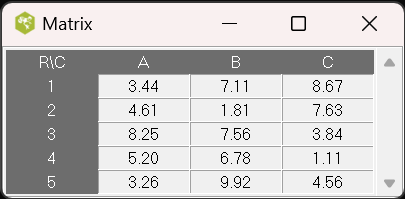
\includegraphics[width=0.4\linewidth]{viewmatrix}
\caption{Interactive table and matrix viewer}
\label{fig:viewdata}
\end{figure}

\clearpage
\section{Plot XY Data}
XY data can be explored graphically with the command \cmdlink{plotXY}. Use the arrow keys or slider to move through the data, and use the scroll wheel on the mouse to switch between data series.
This widget was inspired from ``plotpoints'' on the Tcl wiki: \url{https://wiki.tcl-lang.org/page/A+little+function+plotter}.
\begin{syntax}
\command{plotXY} \$XY \\
plotXY \$X \$Y1 \$Y2 ...
\end{syntax}
\begin{args}
\$XY & Matrix where the first column is X, the second column is Y1, third column Y2, etc. \\
\$X \$Y1 \$Y2 ... & X and Y vectors of the same length, mutually exclusive with \texttt{\$XY}. 
\end{args}
\begin{example}{Creating a figure object}
\begin{lstlisting}
namespace path ::tcl::mathfunc
set x [linsteps 0.01 -10 10]
set y [vmap sin $x]
plotXY $x $y
wob::mainLoop
\end{lstlisting}
\end{example}
\begin{figure}[!htb]
\centering
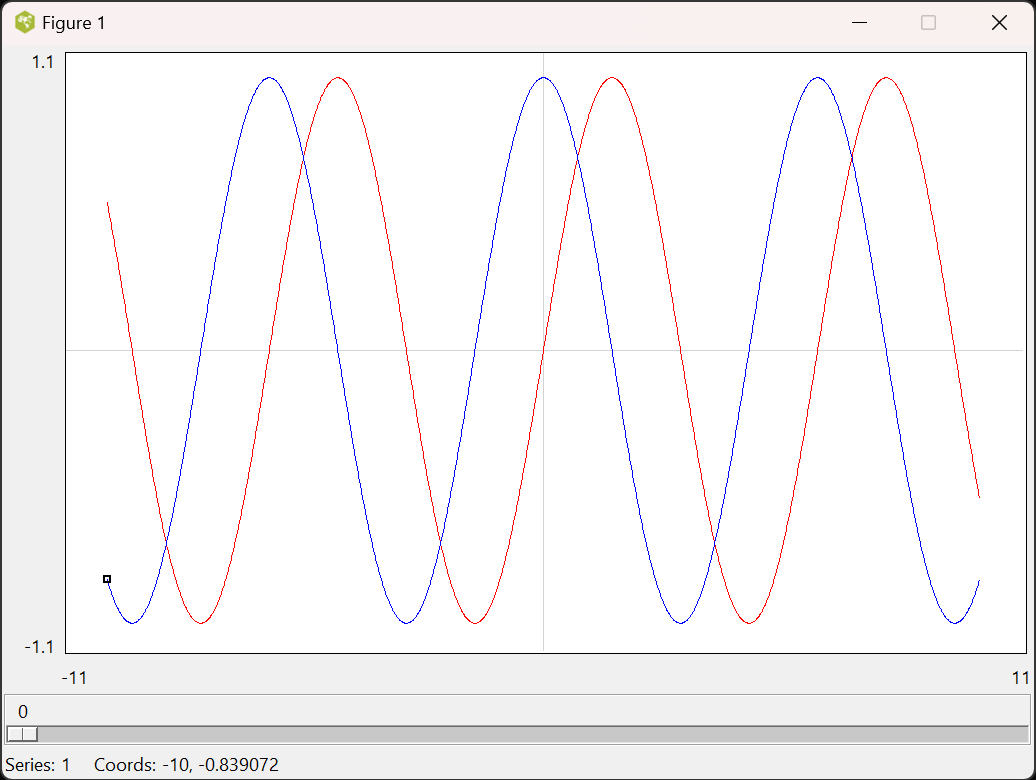
\includegraphics[width=0.7\linewidth]{plot}
\caption{Example XY plot}
\label{fig:plot}
\end{figure}
